% Exemplo: gráfico de barras e de linhas com o pacote pgfplots, com lista própria de gráficos
% Compilar: latexmk -pdf grafico-pgfplots.tex     Testado com: abntex2, pgfplots, TeX Live 2024 ou mais recente
\documentclass[12pt, a4paper, brazilian]{abntex2}
\usepackage[T1]{fontenc}
\usepackage{tikz}
\usepackage{pgfplots}
\pgfplotsset{compat=newest}

%%BEGIN:graficopreambulo
% Float "Gráfico" (a abntex2 não o define): numeração própria e lista de
% gráficos (memoir)
\newfloat{grafico}{lgr}{Gráfico}
\newlistof{listofgraficos}{lgr}{Lista de gráficos}
\newlistentry{grafico}{lgr}{0}       % linha da lista, com pontilhado
\providecommand{\graficoautorefname}{Gráfico}  % nome usado pelo \autoref
% números com vírgula decimal nos eixos e nos rótulos (o padrão é o ponto)
\pgfplotsset{/pgf/number format/use comma}
%%END:graficopreambulo

\begin{document}

O \autoref{gra:barras} compara duas implementações; o \autoref{gra:linhas} mostra a evolução
do tempo de resposta.

%%BEGIN:graficobarras
\begin{grafico}[htbp]
  \caption{Tempo médio de resposta por implementação}\label{gra:barras}
  \centering
  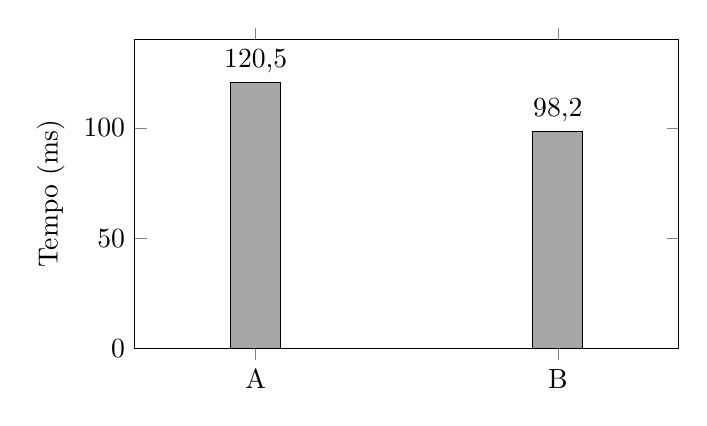
\begin{tikzpicture}
    \begin{axis}[ybar, width=0.7\linewidth, height=5.5cm, bar width=18pt,
        symbolic x coords={A, B}, xtick=data, ymin=0, ymax=140,
        ylabel={Tempo (ms)}, nodes near coords, enlarge x limits=0.4]
      \addplot[fill=black!35] coordinates {(A,120.5) (B,98.2)};
    \end{axis}
  \end{tikzpicture}
  \fonte{Elaborado pelo próprio autor.}
  \nota{Média de 30 execuções.}
\end{grafico}
%%END:graficobarras

%%BEGIN:graficolinhas
\begin{grafico}[htbp]
  \caption{Tempo de resposta por número de usuários simultâneos}
  \label{gra:linhas}
  \centering
  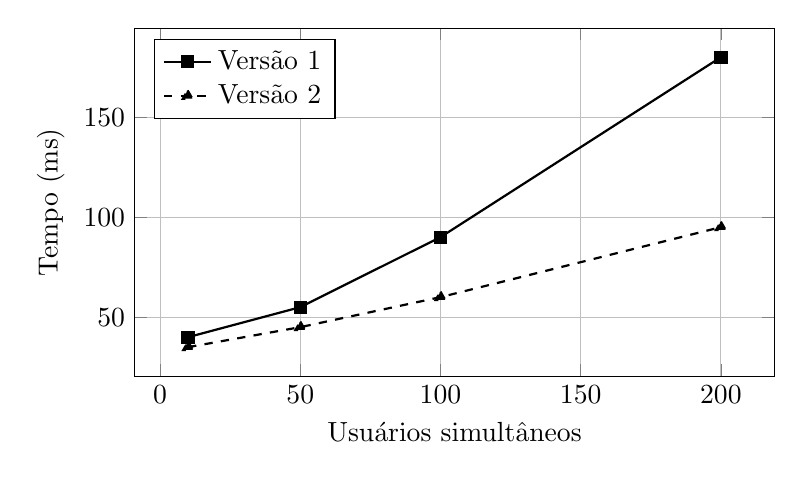
\begin{tikzpicture}
    \begin{axis}[width=0.8\linewidth, height=6cm,
        xlabel={Usuários simultâneos}, ylabel={Tempo (ms)},
        grid=major, legend pos=north west]
      \addplot[mark=square*, thick]
        coordinates {(10,40) (50,55) (100,90) (200,180)};
      \addplot[mark=triangle*, thick, dashed]
        coordinates {(10,35) (50,45) (100,60) (200,95)};
      \legend{Versão 1, Versão 2}
    \end{axis}
  \end{tikzpicture}
  \fonte{Elaborado pelo próprio autor.}
\end{grafico}
%%END:graficolinhas

\end{document}
